\documentclass[12pt,a4paper]{report}
\usepackage{pgfplots}
\usepackage{amsmath}
\usepackage{graphicx}
\usepackage{fancyhdr}
\usepackage{tikz}
\usepackage{multirow}
\usepackage{booktabs}
\usepackage{makecell}

\makeatletter
\renewcommand{\@chapapp}{Week}
\makeatother

\pgfplotsset{compat=1.18}

\title{Fundamental Labs\\Kinematics and Mechatronics}
\author{Prabhnoor Singh Sahni}
\date{\today}

\begin{document}

\maketitle
\tableofcontents

\chapter{LEGO Mindstorms Programming and Mechanism assembly and operation}

\section{Purpose}
\begin{itemize}
    \item Learn basics on kinematics and mechatronics, such as gear and link mechanisms.
    \item Assemble actual mechanisms, move them, and learn how the mechanisms work.
\end{itemize}
\section{Robolab Basic Operation}
We begin our experiments by setting up the computer and starting Robolab. 
Our first program is to rotate a motor.
\subsection{\textbf{Assignment 1}}
\begin{enumerate}
    \item For rotating a motor, we select the appropriate icon for the motor and make the program according to the 
instructions given in the Labs text, Figure~\ref{fig:ass1-1}. 
\begin{figure}[htbp]
    \centering
    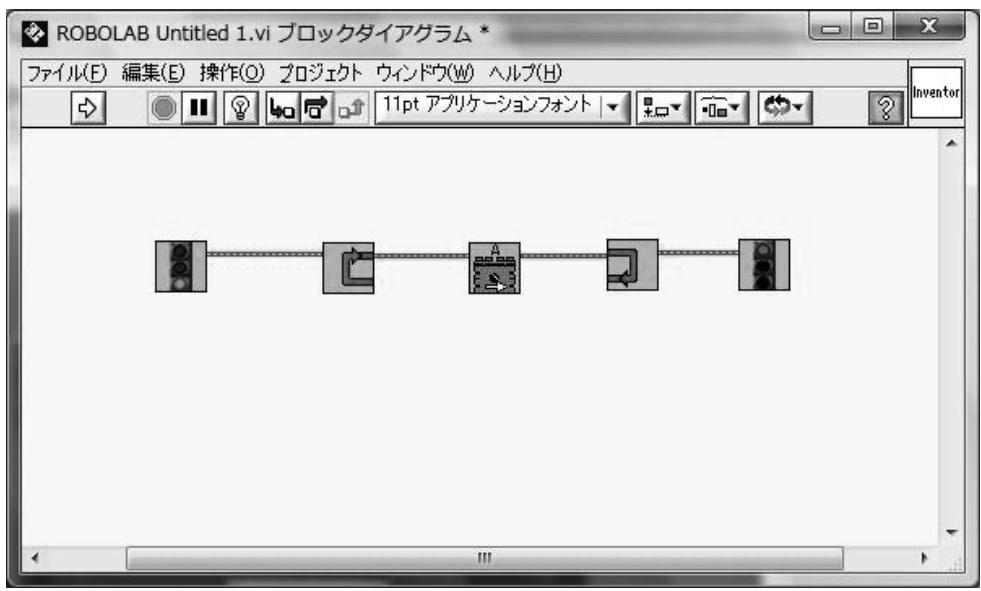
\includegraphics[width=0.7\textwidth]{figures/ass1-1.jpg}
    \caption{Program to rotate a motor eternally}
    \label{fig:ass1-1}
\end{figure}
After connecting the motor to the output of the NXT and after connecting NXT to computer. 
We upload the program and run the NXT. We can confirm the operation of the motor. 
\item Now, we make changes to this program to make the motor rotate and stop when we press and release touch 
    sensor. For this purpose, we use the icon for the touch sensor and add it in the program to get the desired 
    output. 
    Figure~\ref{fig:ass1-2-1} shows the program in Robolab, and Figure~\ref{fig:ass1-2-2} shows the motor along 
    with the touch sensor. 
    \begin{figure}[htbp]
        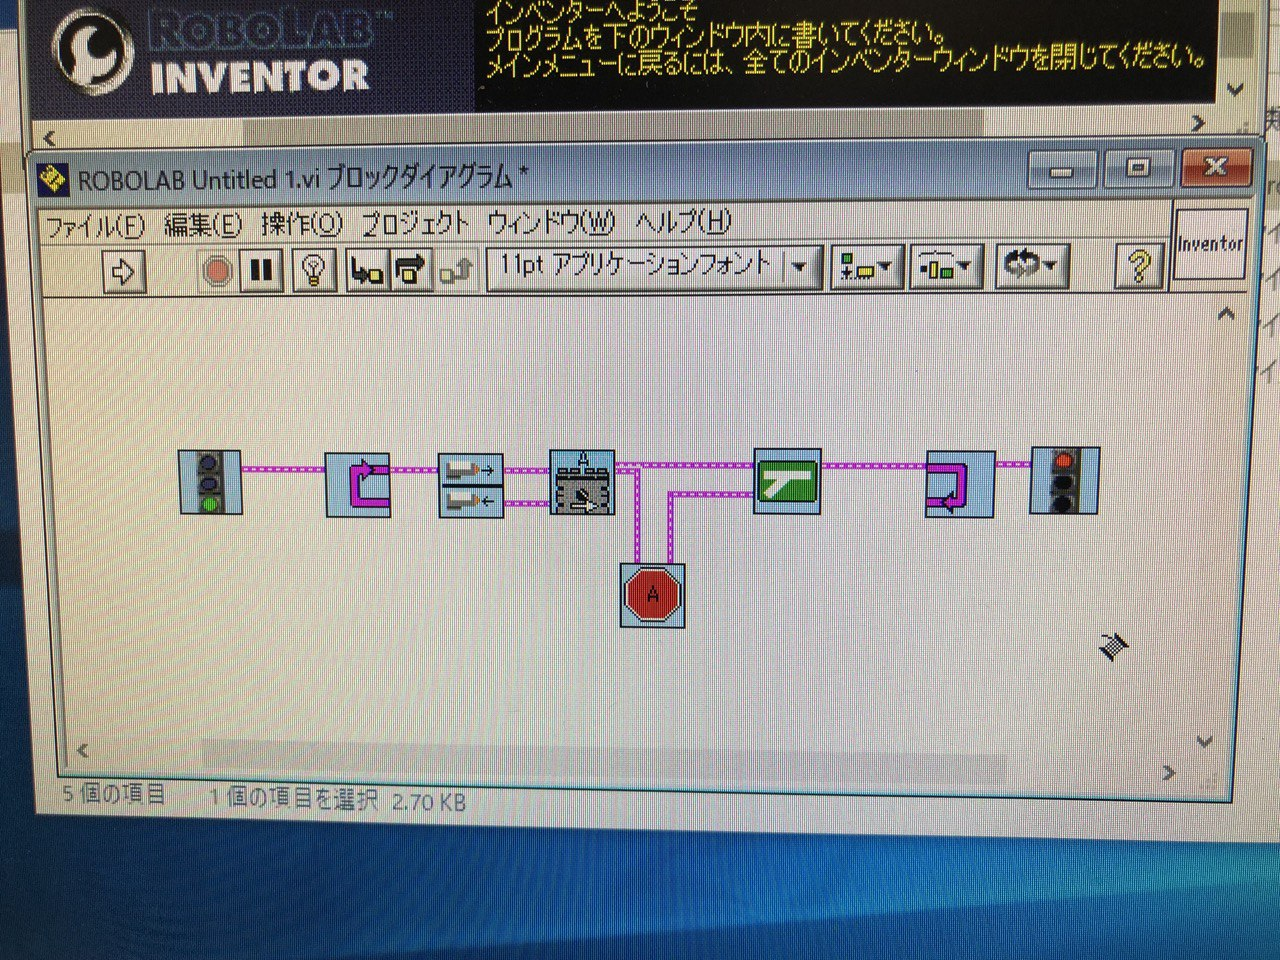
\includegraphics[width=0.7\textwidth]{figures/ass1-2-1.jpg}
        \caption{Program to rotate motor by using a touch sensor.}
        \label{fig:ass1-2-1}
    \end{figure}
    \begin{figure}[htbp]
        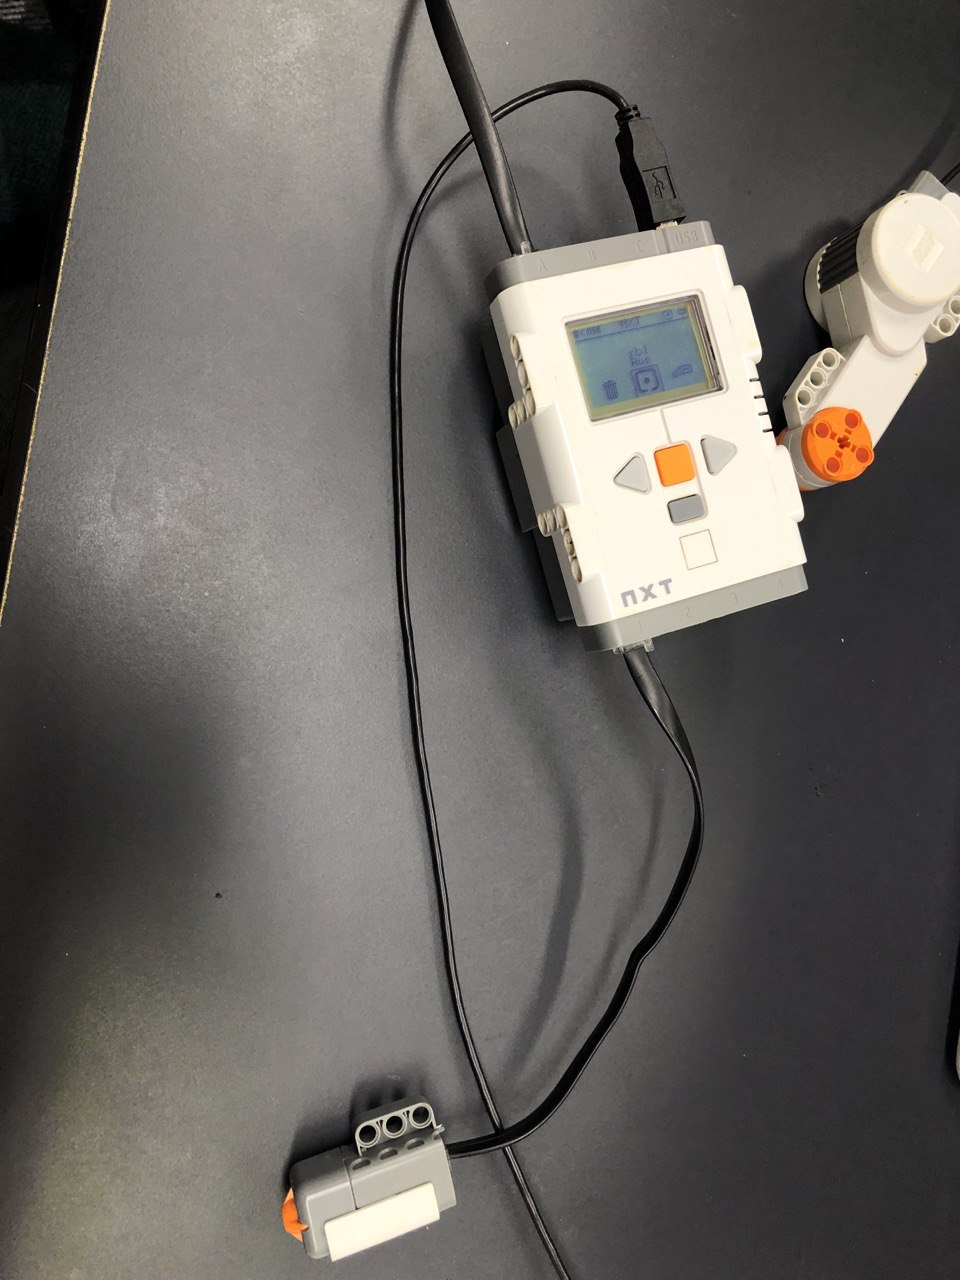
\includegraphics[width=0.7\textwidth]{figures/ass1-2-2.jpg}
        \caption{The physical components when motor is rotated using a touch sensor.}
        \label{fig:ass1-2-2}
    \end{figure}
\item In the next task, we're supposed to make a motor stop and rotate when an optical sensor is directed 
    to face a bright place and a dark place. 
    For this we use the icon for the optical sensor and connect the appropriate terminals to the stop icon. 
    This is in turn connected to the motor as in Figure~\ref{fig:ass1-3-1}. 
    \begin{figure}[htbp]
        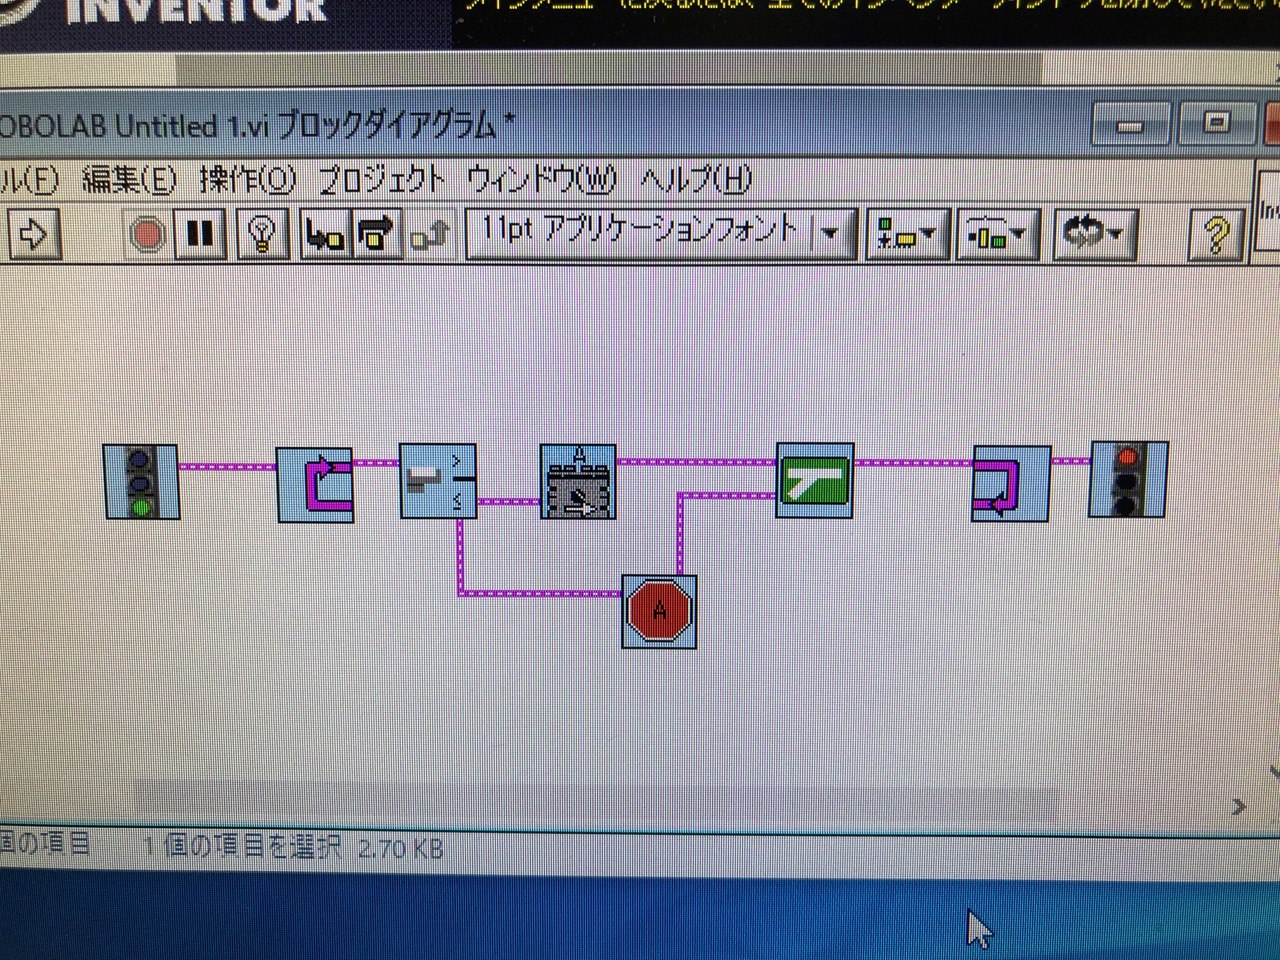
\includegraphics[width=0.7\textwidth]{figures/ass1-3-1.jpg}
        \caption{Program for rotating motor depending on input from optical sensor}\label{fig:ass1-3-1}
    \end{figure}
    \begin{figure}[htbp]
        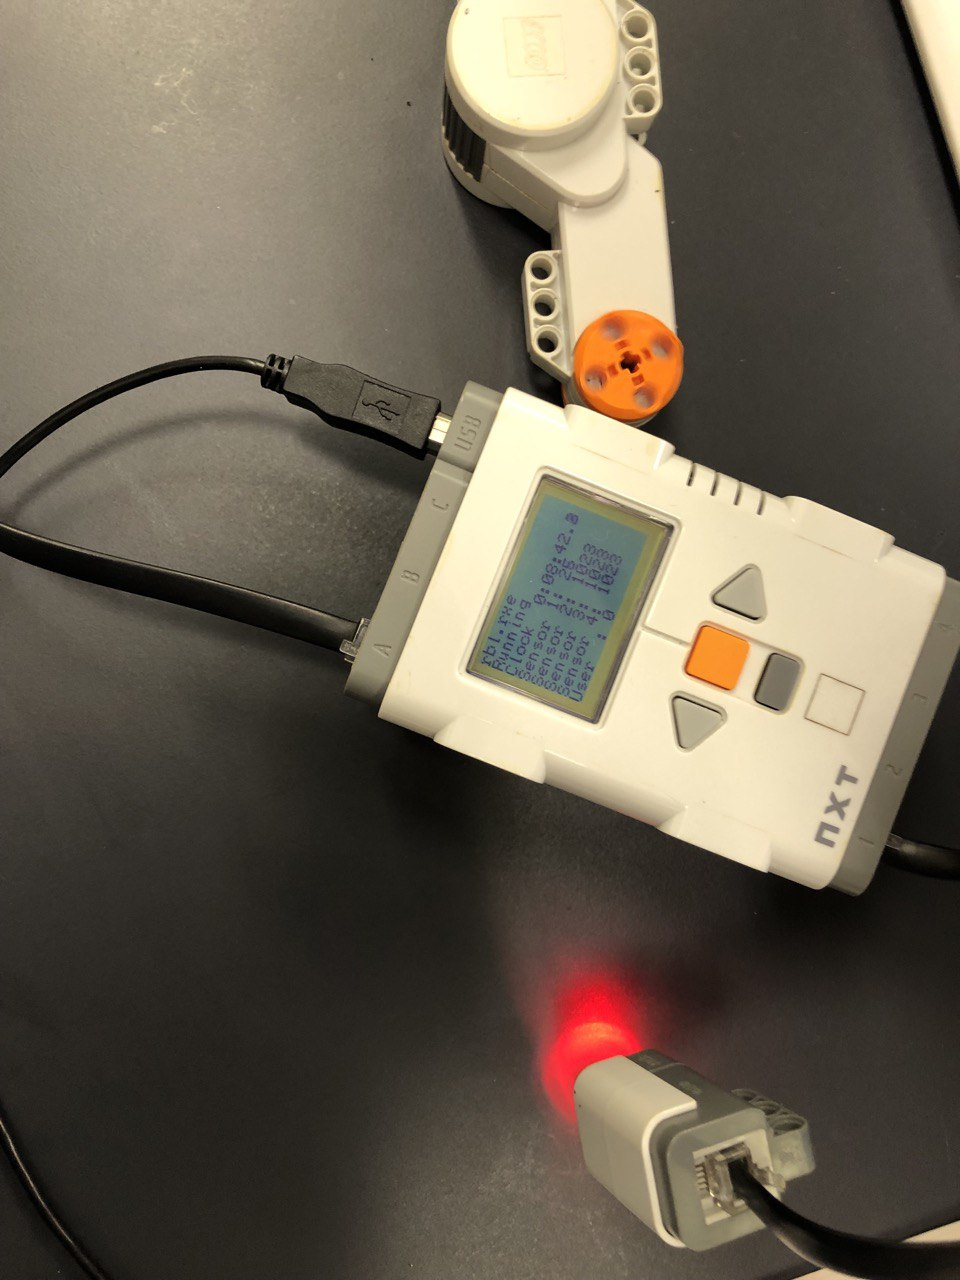
\includegraphics[width=0.7\textwidth]{figures/ass1-3-2.jpg}
        \caption{Physical components when optical sensor is used as input to rotate motor.}\label{fig:ass1-3-2}
    \end{figure}
    We were able to confirm the operation of this assignment. We saw that the motor was rotating the optical 
    sensor was directed to a white paper and the motor stopped when the sensor was directed to the black table. 
\end{enumerate}
\subsection{\textbf{Assignment 2}}
In this assignment, we were required to create a program such that when the touch sensor is pressed, 
the motor starts making reverse rotations. 
For this purpose, we use the wait for icon of the sensors. The icon for touch sensor waits for the input, 
and based on that it makes the motor rotate either in forward or reverse direction. We have to use two of 
these sensors to make sure that the flip between forward and reverse is recurrent.  
Then we create the program on the computer, which can be seen in Figure~\ref{fig:ass2-1}. 
\begin{figure}[htbp]
    \centering
    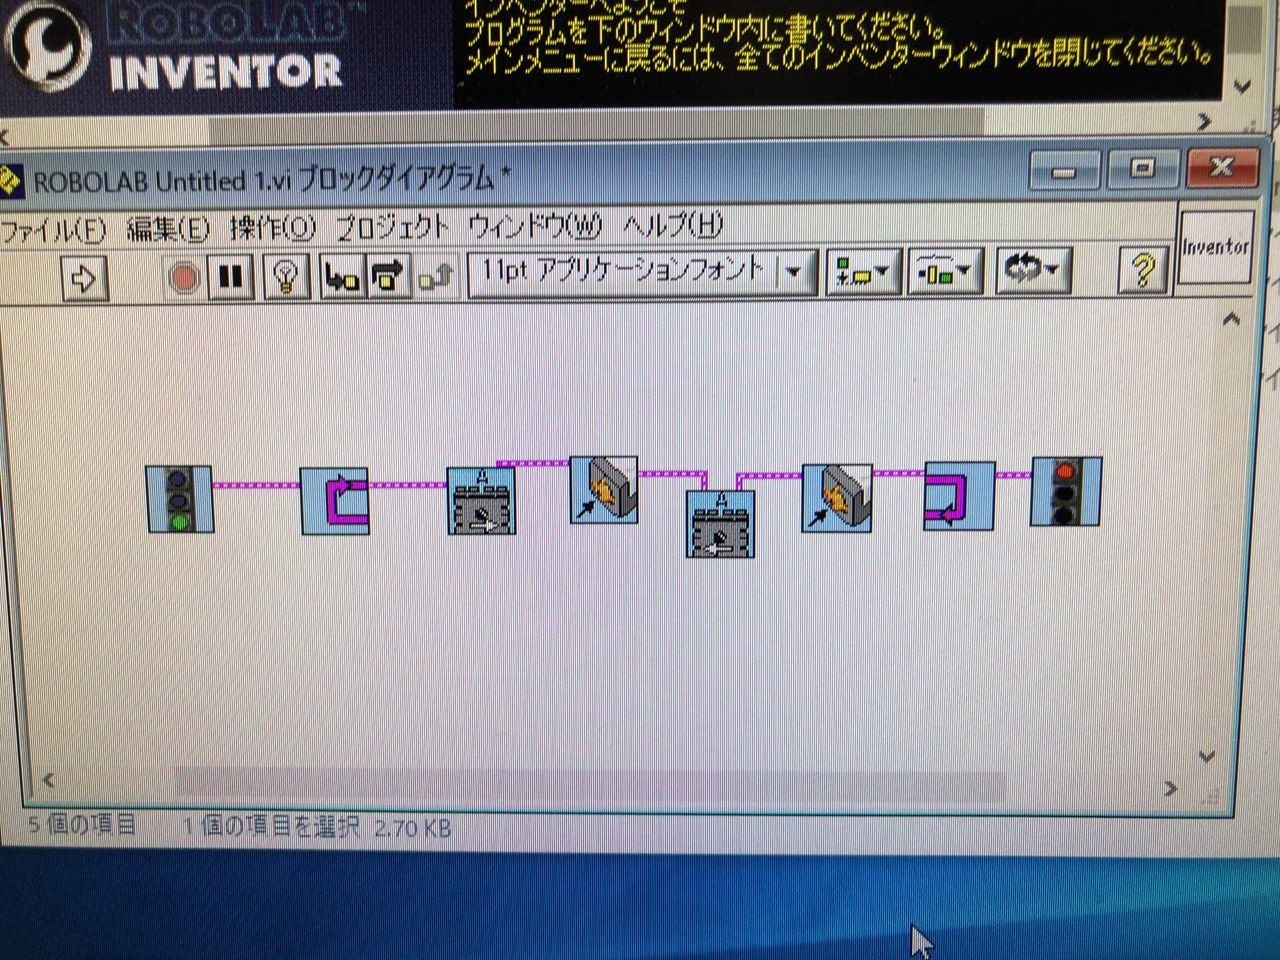
\includegraphics[width=0.7\textwidth]{figures/ass2-1.jpg}
    \caption{Program to rotate a motor either in forward or reverse direction based on the number of times the touch sensor is pressed.}
    \label{fig:ass2-1}
\end{figure}
We can confirm the operation of our motor and touch sensor once we pass the code into the NXT. 

\subsection{\textbf{Assignment 3}}
In this assignment we use a distnace sensor and motor to create a program so that when the distance with the 
wall is near, the motor rotates; when the distance is in the middle, the motor stops and when the 
distance is far, the motor shows reverse rotations. 
For this assignment, we have used two distance sensors, a stop icon, two icons for defining constant integer 
values used to check distance, branches and two motors (one for reverse, other for forward). 
Basically, for the program, we first set particular distance values. Since the sensor gives output in centimetres. 
We set that if the output is more than 20 cm, the distance is far; if it's less than 10 cm, the distance is near 
and if it's between 10 cm and 20 cm, the distance is in the middle. Using this logic, we make a flowchart showing 
the process as in Figure~\ref{fig:ass3-1}. And then, using the flowchart it becomes pretty straightforward to 
create the program on the computer. The program is as in Figure~\ref{fig:ass3-2}. 
\begin{figure}[htbp]
    \centering
    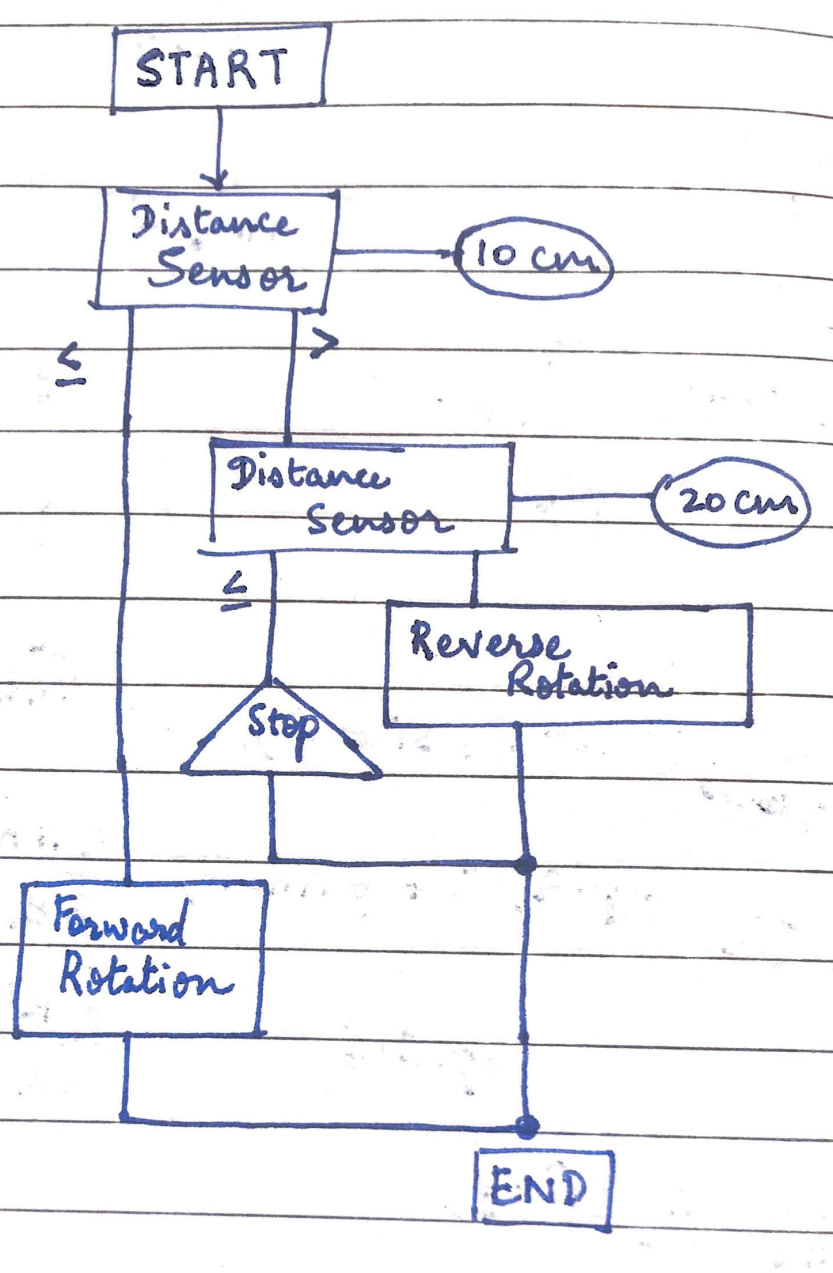
\includegraphics[width=0.7\textwidth]{figures/ass3-1.jpg}
    \caption{Flowchart explaining the process of motor rotation through distance sensor. It shows that the program 
    starts by checking the data from the distance sensor. If data is less than or equal to 10 cm, it moves 
    to rotating the motor. If it's more than 10 cm, it goes through another check to determine if it's more than 
    20 cm. Depending on this output, it either stops or rotates the motor.}
    \label{fig:ass3-1}
\end{figure}
\begin{figure}[htbp]
    \centering
    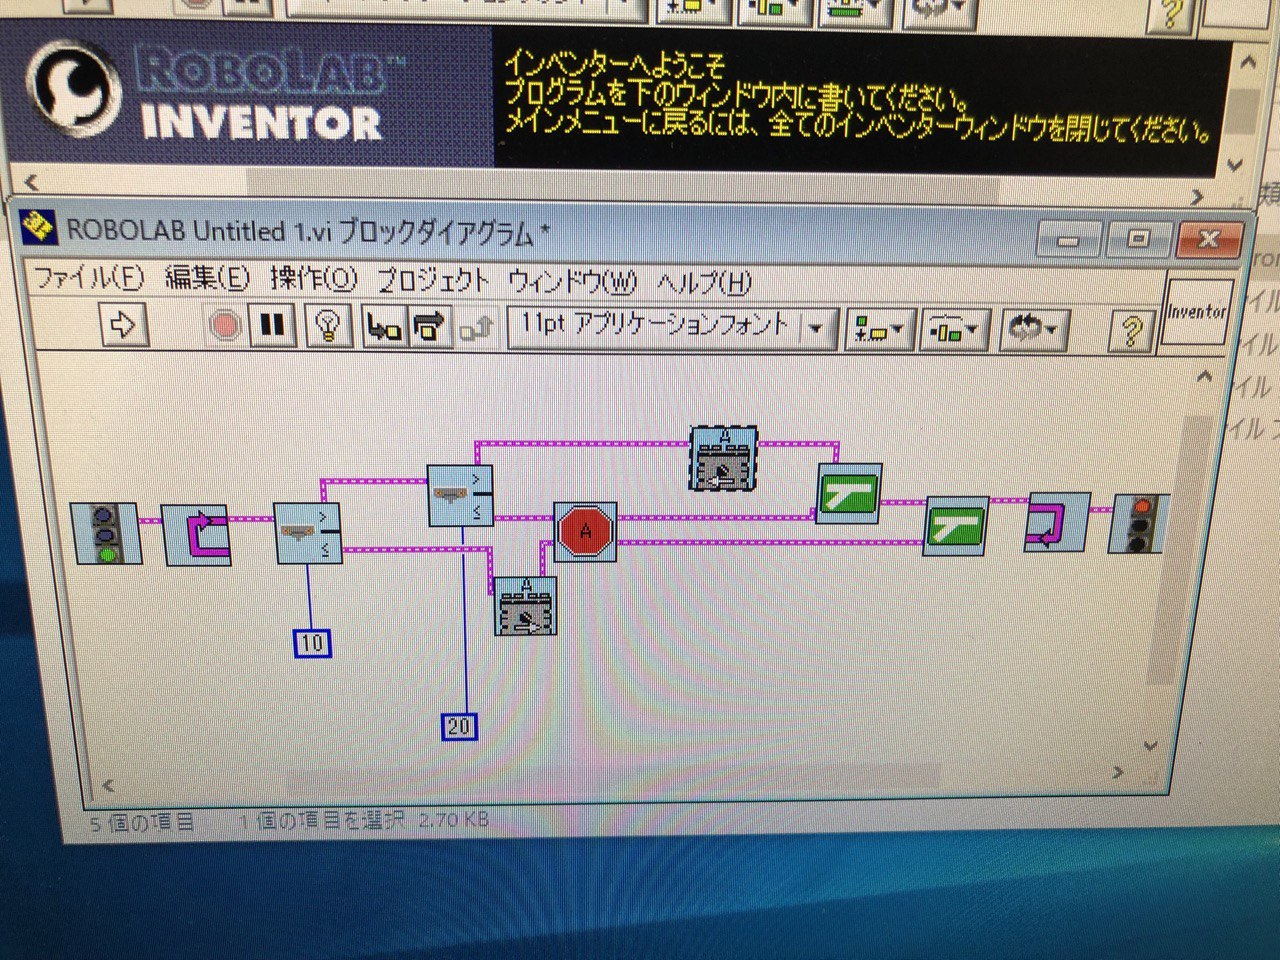
\includegraphics[width=0.7\textwidth]{figures/ass3-2.jpg}
    \caption{Program to rotate a motor when distance is near, stop when distance is middle and reverse rotations 
    when distance is far.}
    \label{fig:ass3-2}
\end{figure}
We confirm the operation after pushing code to the NXT and running it. 

\section{Rotational velocity and force conversion of flat gear-based systems}
In this section we proceed to understand rotational velocity and force conversion in multigear systems. 
In a multigear system, gears with different numbers of teeth rotate at different speeds. The basic principle is that larger gears (more teeth) rotate more slowly but produce more torque, while smaller gears (fewer teeth) rotate faster but with less torque.
\subsection{\textbf{Assignment 4}}
In the three assignments described, there are differences in rotational velocity and force depending on the configuration 
of the gears and their sizes.\\
In the first experiment when we are independently rotating the gears the rotational speeds and force are also independent.
Now, in the second experiment we drive the small gear with motor, while the larger gear. Let the properties denoted by "1" 
represent the smaller gear and those denoted by "2", the larger gear.\\
Case 1: \textbf{Motor on small gear}\\
Let time go from t=0 seconds to t=t seconds. In this time, 
\begin{align}
    \text{(Distance covered by a teeth of gear 1)} &= \text{(Distance covered by a teeth of gear 2)}, \\
                                                       &= 2\pi r_2.
\end{align}
This shows that Gear 1 does \(\frac{r_2}{r_1}\) rotations in t seconds and Gear 2 does 1 rotation. 
Thus, 
\begin{align}
    \omega_1&=\frac{r_2}{r_1} \frac{1}{t} rot/s,\\
    \omega_2 &= \frac{1}{t} rot/s, \\
    \frac{\omega_1}{\omega_2}&=\frac{r_2}{r_1}\\
    \Rightarrow \omega_1&=\frac{r_2}{r_1} \omega_2\\
    \text{or } \omega_2 &= \frac{r_1}{r_2}\omega_1.
\end{align}
where \(\omega\) is angular velocity. \\
Now, moving to torque, we know that Torque \(\tau = \mathbf{r} \times \mathbf{F}\).
Thus, (considering only magnitudes),
\begin{align}
    \tau_1 &= r_1F,\\
    \tau_2 &= r_2F,\\
    \Rightarrow \tau_2 &= \frac{r_2}{r_1} \tau_1.
\end{align}
The term \(\frac{r_2}{r_1}\) is called the reduction ratio and its inverse, \(\frac{r_1}{r_2}\) is called the reciprocal 
reduction ratio. 
The \textbf{reduction ratio} refers to how much the rotational speed or torque is decreased (or increased) from the 
input to the output.
Case 2: \textbf{Motor on big gear}\\
Just like Case 1, we have:
\begin{align}
    \text{(Distance covered by a teeth of gear 1)} &= \text{(Distance covered by a teeth of gear 2)}, \\
                                                       &= 2\pi r_2.
\end{align}
This shows that Gear 1 does \(\frac{r_2}{r_1}\) rotations in t seconds and Gear 2 does 1 rotation. 
Thus, 
\begin{align}
    \omega_1&=\frac{r_2}{r_1} \frac{1}{t} rot/s,\\
    \omega_2 &= \frac{1}{t} rot/s, \\
    \omega_1 &= \frac{r_2}{r_1}\omega_2.
\end{align}
Also,
\begin{equation}
    \Rightarrow \tau_1 = \frac{r_1}{r_2} \tau_2.
\end{equation}

\subsection{\textbf{Assignment 5}}
Now, unlike our two gear system in last assignment, we prepare a three gear system. 
Since we know the reduction ratio and the relationship between two gears from the previous assignment, we can directly 
use those results to understand this problem. \\
Consider the three gears denoted by "1","2" and "3". Let \(\omega\) be angular velocity and \(r\) be radius. \\
\begin{align}
    \omega_2&=\frac{r_1}{r_2}\omega_1,\\
    \omega_3&=\frac{r_2}{r_3}\omega_2,\\
    \Rightarrow \omega_3&=\frac{r_1}{r_3}\omega_1.\\
\end{align}
Also, 
\begin{align}
    \tau_2&=\frac{r_2}{r_1}\tau_1,\\
    \tau_3&=\frac{r_3}{r_2}\tau_2,\\
    \Rightarrow \tau_3&=\frac{r_3}{r_1}\tau_1.
\end{align}
We can see that Gear 1 and Gear 3 are rotating in the same direction. Gear 3 rotates as if Gear 2 does not exist. 
Its angular velocity and torque depends completely on Gear 1. 
\subsection{\textbf{Assignment 6}}
In order to achieve a very large deceleration ratio we want to make sure that the terms do not get cancelled. 
So if we can make the gears not touch by their teeth, but instead have same characteristics as the source gear (one driven by 
motor). We can do this by keeping two or more gears on top of each other, i.e. two gears driven by same motor. 
See Figure~\ref{fig:ass6}.\\
\begin{figure}
            \centering
    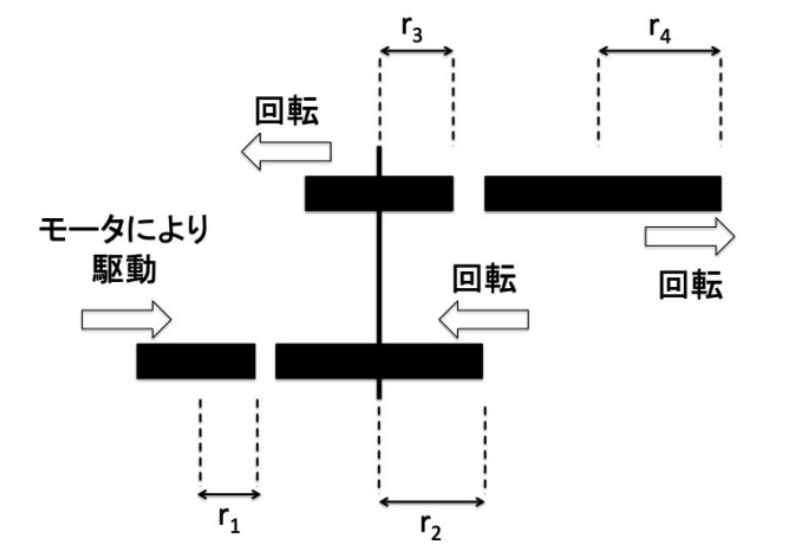
\includegraphics[width=0.7\textwidth]{figures/ass6.jpg}
    \caption{Multiple Flat Gear system}
    \label{fig:ass6}
\end{figure}
\begin{align}
    \omega_1=\frac{r_2}{r_1}\omega_2 &, \omega_4=\frac{r_3}{r_4}\omega_3;\\
    \text{we know, } \omega_3&=\omega_2.\\
    \text{Thus, } \omega_4&=\frac{r_3r_1}{r_4r_2}\omega_1.
\end{align}
Also for torque, using a similar approach we get:
\begin{equation}
    \tau_4=\frac{r_4r_2}{r_3r_1}\tau_1
\end{equation}
Hence, we have achieved a large deceleration/reduction ratio where the terms do not get cancelled. 
This type of system has many uses. 

\subsection{\textbf{Assignment 7}}
"Backlash" refers to the amount of clearance or play between mating gears. It is the relative motion or movement between 
gears when they change direction of rotation, particularly when transitioning from driving to coasting or vice versa.
Generally, there is no problem when the gears are continuously rotating in some direction. 
The problem arises when the direction of rotation is reversed or changed.\\
When the motion is reversed, the clearance between the gear teeth causes a brief moment where the gears disengage before 
they engage again in the opposite direction. This can lead to several issues.\\
\begin{itemize}
    \item Backlash can introduce inaccuracies and imprecision in the movement of mechanical systems. 
    \item It can cause mechanical wear and tear. 
    \item It has an overall impact on performance. 
\end{itemize}

\section{Bevel gear, worm gear-based rotational direction conversion}
For this section, we assembled a mechanism consisting of a motor, bevel gear and worm gear based on the instructions 
provided. The final assembled structure is as shown in Figure~\ref{fig:ass8}. 
\begin{figure}[htbp]
            \centering
    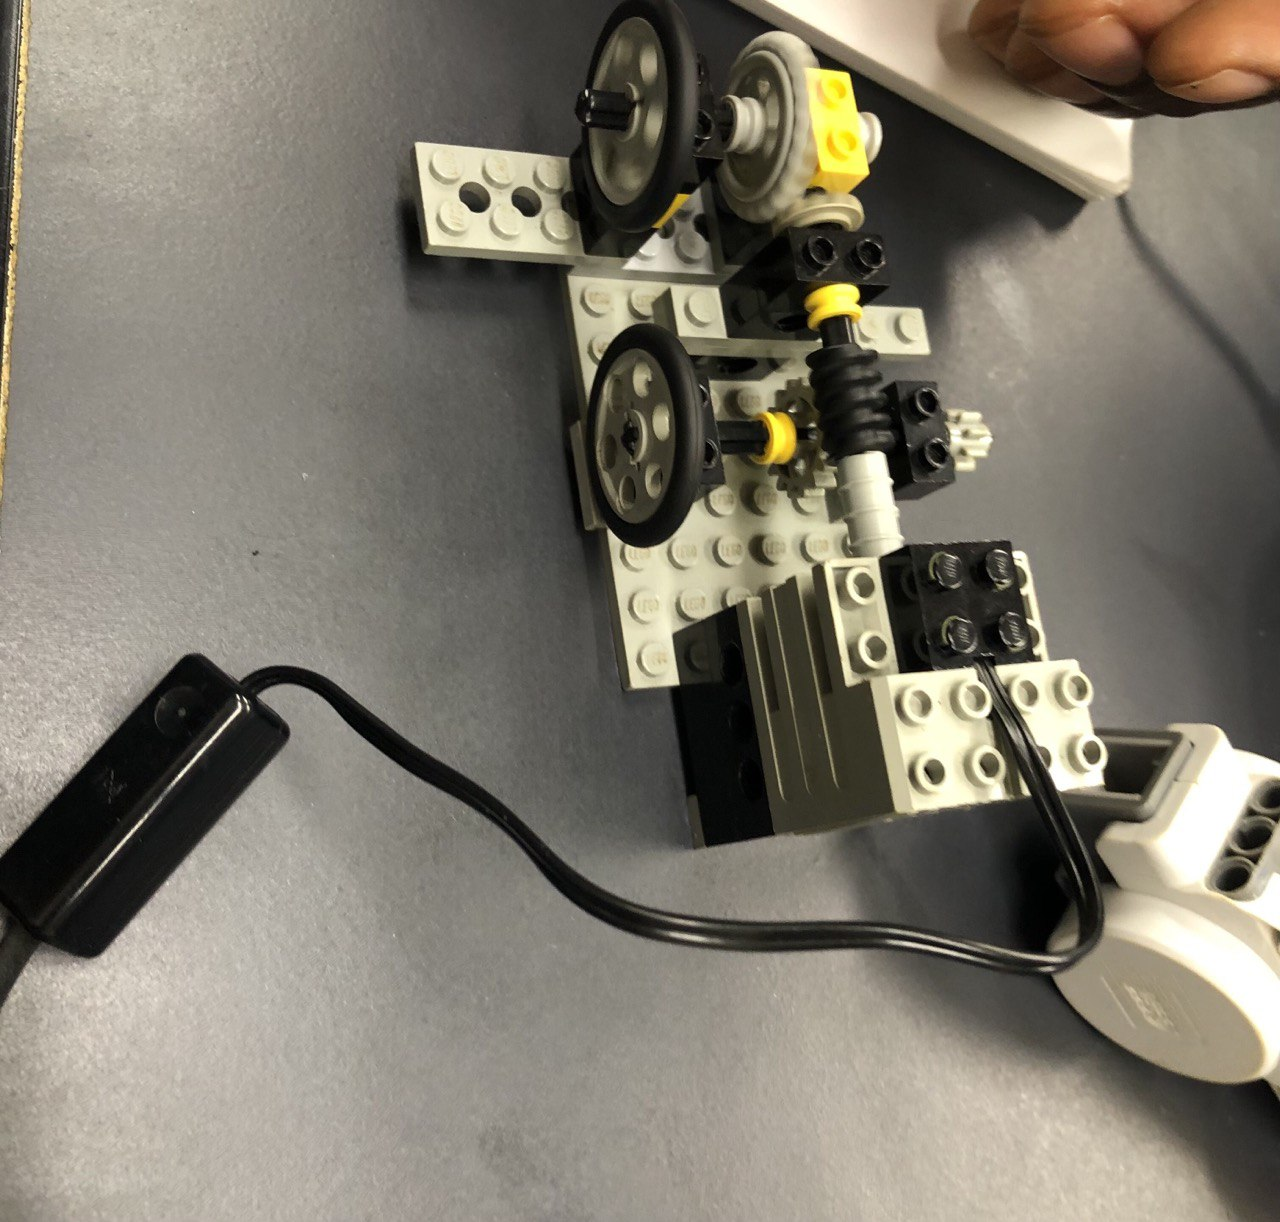
\includegraphics[width=0.7\textwidth]{figures/ass8}
    \caption{Bevel gear, worm gear-based rotational axis conversion mechanism}
    \label{fig:ass8}
\end{figure}
\subsection{\textbf{Assignment 8}}
When we do not know the properties like radius or angular velocity in a physical system, how does one find the recution 
ratio? Reduction ratio is an intrinsic property of gears. Thus, another measure of the reduction ratio can be by using number 
of teeth. We see that the reduction ratio or deceleration ratio, given by \(\frac{r_2}{r_1}\) can also be written as 
\[\frac{n_2}{n_1}\] where n is the number of teeth in the gear. 
This is true because the number of teeth on a gear is directly proportional to the radius. \\
For our system, for the bevel gear, since the two gears had 12 and 24 teeths. Thus \(n_1=12\) and \(n_2=24\). So 
reduction ratio \(= \frac{n_2}{n_1}=2\).\\
Now, for the worm gear. A worm gear has n teeth. So it will have n rotations. 
Let the angular velocity of the worm gear in our system be denoted by \(\omega_3\), then 
\begin{align}
    \frac{\omega_4}{\omega_3}&=\frac{1}{n},\\
    \omega_4&=\frac{1}{n}\omega_3.
\end{align}
Also, 
\begin{align}
    \frac{\tau_4}{\tau_3}&=\frac{r_4}{r_3}\\
                         &=\frac{n_4}{n_3}\\
                         &=n (\text{because }n_3=1\text{ and }n_4=n).\\
    \Rightarrow \tau_4 &= n\tau_3.
\end{align}
Thus reduction ratio is n=16 (for worm gear).

\subsection{\textbf{Assignment 9}}
There is a force applied on the worm gear. This force has two components, \(f cos(\theta) \text{ and } f sin(\theta)\) since 
it is applied at an angle \(\theta\). Now, due to contact, there also exists a friction force (\(f'\)), opposite to the 
motion. Let \(\mu\) be the coefficient of friction. \\
We notice that in this motion there are two conditions-- not rotating and rotating,let's discuss them in detail. \\
\textbf{Not Rotating Condition}\\
The gear does not rotate when the force on the worm gear is unable to overcome the force of static friction. 
\begin{align}
    f sin(\theta) &\leq f' = \mu N = \mu f cos(\theta)\\
    \text{Thus, } tan(\theta) &\leq \mu 
\end{align}
where \(N\) is the normal force. \\
See Figure~\ref{fig:ass9}. \\
\begin{figure}[htbp]
            \centering
    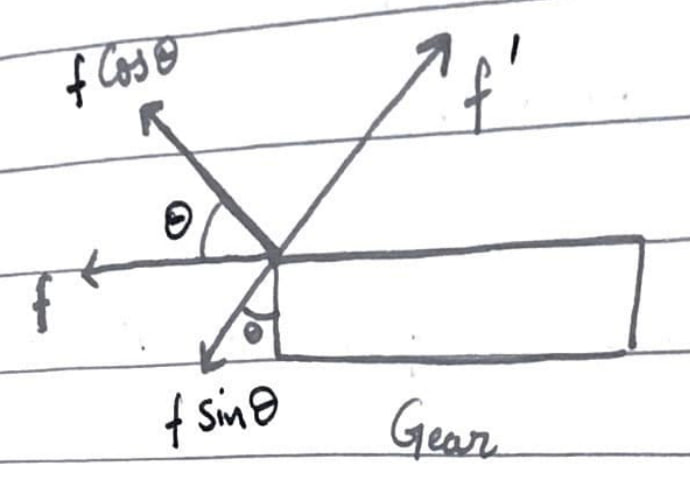
\includegraphics[width=0.7\textwidth]{figures/ass9}
    \caption{Free Body Diagram of a worm gear illustrating the various forces.}
    \label{fig:ass9}
\end{figure}
\textbf{Rotating Condition}\\
The gear will rotate when the force is large enough to overcome the force of friction.\\ 
\begin{align}
    f sin(\theta) &\geq f' = \mu N = \mu f cos(\theta)\\
    \text{Thus, } tan(\theta) &\geq \mu 
\end{align}
Lastly, as we know \(0 \leq \mu \leq 1\), thus, if \(\theta=45^{\circ}\) the gear will rotate regardless of \(\mu\). 
Thus, we can understand the role of friction and angle played in the rotation of the worm gear. 

\chapter{Parallel four-link mechanism and Motion Conversion}
\section{Parallel four-link mechanism}
This week we begin by understanding the working of a parallel four-link mechanism. 
The parallel four-link mechanism is a mechanical system comprising four rigid links connected by revolute joints, 
forming a closed-loop structure. This mechanism offers advantages such as symmetrical motion, predictable kinematics, 
and efficient power distribution.
\subsection{\textbf{Assignment 10}}
Here, we will derive the coordinates of the hand position of the parallel four links. 
From Figure~\ref{fig:ass10}, we can see that: 
\begin{align}
    \vec{OD} &= \vec{OA} + \vec{AB} + \vec{BD},\\
    x &= L_1 cos(\theta_1) + L_2 cos(\theta_2)+L_3cos(\theta_1+\pi)\\
    y &= L_1sin(\theta_1) + L_2 sin(\theta_2) +L_3sin(\theta_1+\pi)
\end{align}
We now substitute from the identities for sum of angles of Cos and Sin.
\begin{align}
    x &= (L_1-L_3)cos(\theta_1)+L_2cos(\theta_2)\\
    y &= (L_1-L_3)sin(\theta_1)+L_2sin(\theta_2)
\end{align}
\begin{figure}[htbp]
            \centering
    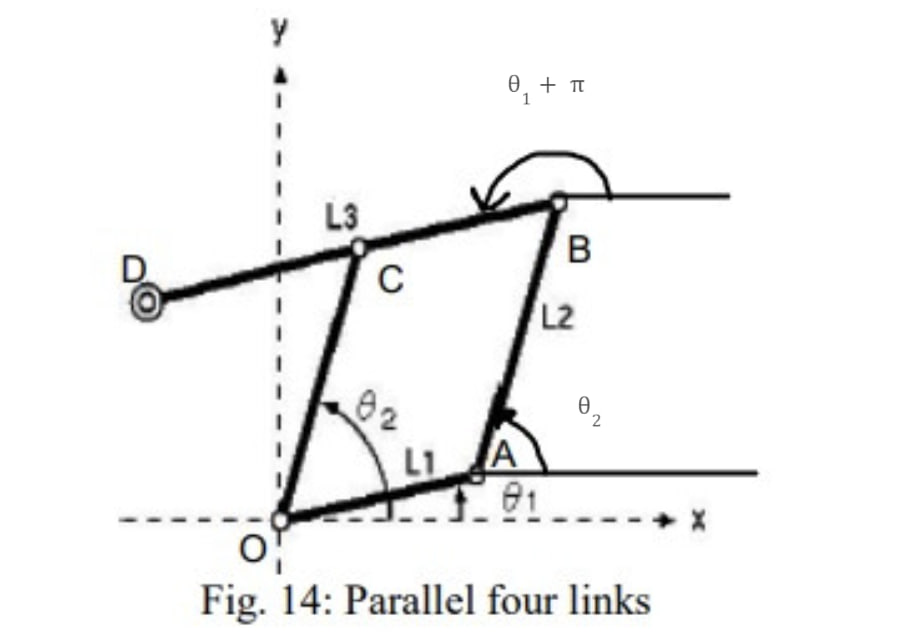
\includegraphics[width=0.7\textwidth]{figures/ass10}
    \caption{Parallel four links diagram}
    \label{fig:ass10}
\end{figure}

\subsection{\textbf{Assignment 11}}
In this section, we analyze the tip operation of a parallel four-bar linkage, focusing on its behavior when the angles between the links are set to \(90^{\circ}\). \\
We begin by setting all angles in the parallel four-bar linkage to 90°, effectively transforming the linkage into a rectangular
shape. See the part labelled as base in Figure~\ref{fig:ass11}. 
Using graph paper, we record the path traced by the tip of the linkage when rotating only the top gear from this orientation. 
Similarly, we record the path when rotating only the bottom gear. \\
We can see the path labelled in Figure~\ref{fig:ass11} as "Only Top Gear", which is obtained when rotating only the top gear. 
We look at the path relative to the base and we can understand the characteristics. Also, we are able to realise the 
position of the centre of the arc that is drawn when tracing this path. We can see the position of the centre right at the 
joining of the link. It is at the joint closest to the pencil. This position is labelled in the figure. \\
Further, we see the arc traced by the rotation of only the Bottom Gear, marked in Figure~\ref{fig:ass11} as "Only Bottom Gear". 
The centre of this circle can be realised by looking at the entire structure and relating the centre of the circle of the arc of 
the rotation of only the top gear. We look at the intersection of the two arcs and with that we're able to find the centre of 
the second circle. \\
\begin{figure}[htbp]
            \centering
    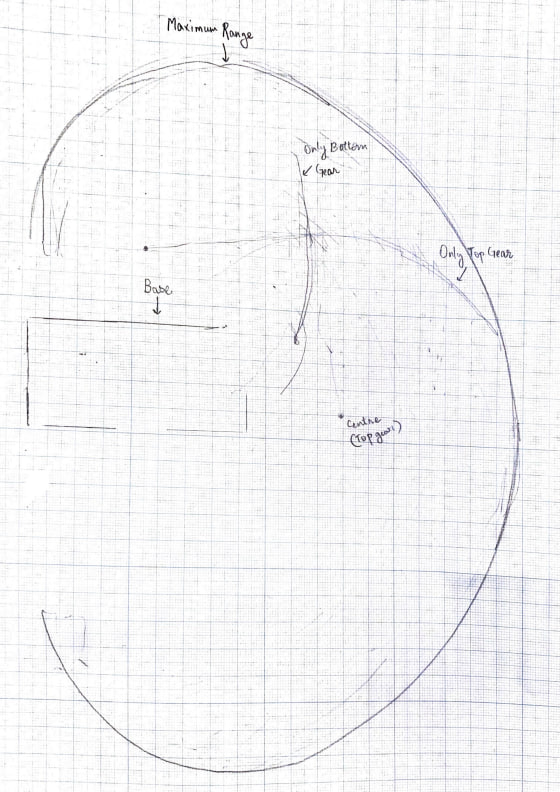
\includegraphics[width=\textwidth]{figures/ass11}
    \caption{Record of the tip operation of the parallel four links on a graph paper.}
    \label{fig:ass11}
\end{figure}
\subsubsection{Why is the range of this not a proper circle?}
There is interference between the base and the links, and this causes the range to be an "improper" circle. 
\subsection{\textbf{Assignment 12}}
When using such a mechanism, there are numerous benefits. Yes, it is indeed possible to place only one motor 
which will enable us to drive both the gears. \\
The obvious advantage is that this mechanism does not need a second motor, as already established. 
Further, By placing the motor on a base that is separate from the link joints, there is greater flexibility in motor selection. 
Motors can be chosen based on their specific performance characteristics without being limited by size and weight constraints 
imposed by the link joints. \\
A crucial advantage in this mechanism is of efficient power distribution. 
Separating the motor from the link joints allows for better distribution of power within the mechanism.
This can lead to reduced energy consumption, as power can be transmitted more directly to the gears without the added 
weight and inertia of the motor affecting the movement of the link joints.\\
Moreover, it also provides us with a greater range of motion because there is only one motor. It also helps in cable management as 
only one cable can be used to connect to the motor. This improve efficiency.
Since the arm does not have a motor, the centralised power delivery system will not fail. It reduces failure.\\
\textbf{Disadvantages of Placing Motor on link-joint sections}\\
Firstly, mounting the motor directly on the link joint sections adds additional weight and inertia to the mechanism. 
This can result in slower response times and reduced efficiency, especially in applications requiring rapid or precise movements.\\
The space available on the link joint sections may be limited, making it challenging to install larger or more powerful motors. 
This limitation can restrict the performance capabilities of the mechanism and limit its potential applications.\\
Placing the motor on the link joint sections increases the risk of interference with the movement of the mechanism. 
The motor's size and positioning may restrict the range of motion or cause unwanted friction or obstruction, leading to 
reduced reliability and performance.\\
\textbf{"non-parallel" four-link Mechanism}\\
To transform the parallel four-link mechanism into a non-parallel configuration, we can modify the lengths of the 
links such that they are no longer parallel. Rotating this modified mechanism will result in a different motion compared 
to the original parallel configuration. Specifically, the trajectory of the tip or end effector will vary, potentially leading 
to different kinematic behaviors and applications. Experimentation with different link lengths and configurations can provide 
insights into the versatility and adaptability of four-link mechanisms for various engineering tasks.\\

\subsection{\textbf{Assignment 13}}
In a parallel four-link mechanism, the motion of the link tips tends to be symmetrical when rotating the top and bottom gears. 
This symmetry arises from the geometric arrangement of the links and joints, resulting in predictable and balanced movement 
patterns.\\
Moreover, the range of movement of the link tips remains relatively consistent across different configurations of the parallel 
four-link mechanism. This is because the parallel arrangement of the links constrains the motion within a certain range, 
providing stability and predictability in operation.\\
\textbf{Advantages of the Parallel Four-Link Mechanism:}\\
The parallel arrangement of the links in the four-link mechanism facilitates predictable kinematics, 
making it easier to design and control. Symmetrical motion patterns and consistent range of movement 
contribute to the reliability and stability of the mechanism in various applications.\\
Lastly, the geometric simplicity of the parallel four-link mechanism simplifies design and analysis processes. 
Engineers can leverage symmetrical motion characteristics and consistent range of movement to optimize performance 
and address specific requirements without the added complexity associated with non-parallel configurations. It allows 
for better and simpler calculation. \\

\section{Motion Conversion}
In this section we examine mechanisms for converting rotational motion into other forms of motion, like reciprocal or 
straight line motion. 
\subsection{\textbf{Assignment 14}}
We have created the following three mechanisms for converting rotational motion of a motor into different types of reciprocating 
motion.
\begin{itemize}
    \item Oscillation Mechanism (Figure~\ref{fig:ass14-3})
    \begin{figure}[htbp]
        \centering
        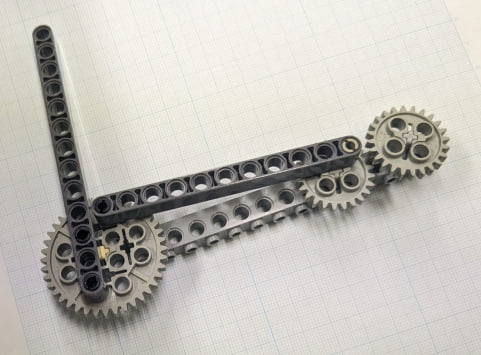
\includegraphics[width=0.5\textwidth]{figures/ass14-3}
        \caption{Figure illustrating the mechanism created for showing reciprocating oscillation motion.}
        \label{fig:ass14-3}
    \end{figure}

    \item Cam Mechanism (Figure~\ref{fig:ass14-2})\\
    A cam mechanism consists of a cam and a follower. The cam is a specially shaped component mounted on a rotating shaft, 
    while the follower rides on the cam's surface. As the cam rotates, it imparts motion to the follower, converting rotary 
    motion into reciprocating or oscillating motion.
    \begin{figure}[htbp]
        \centering
        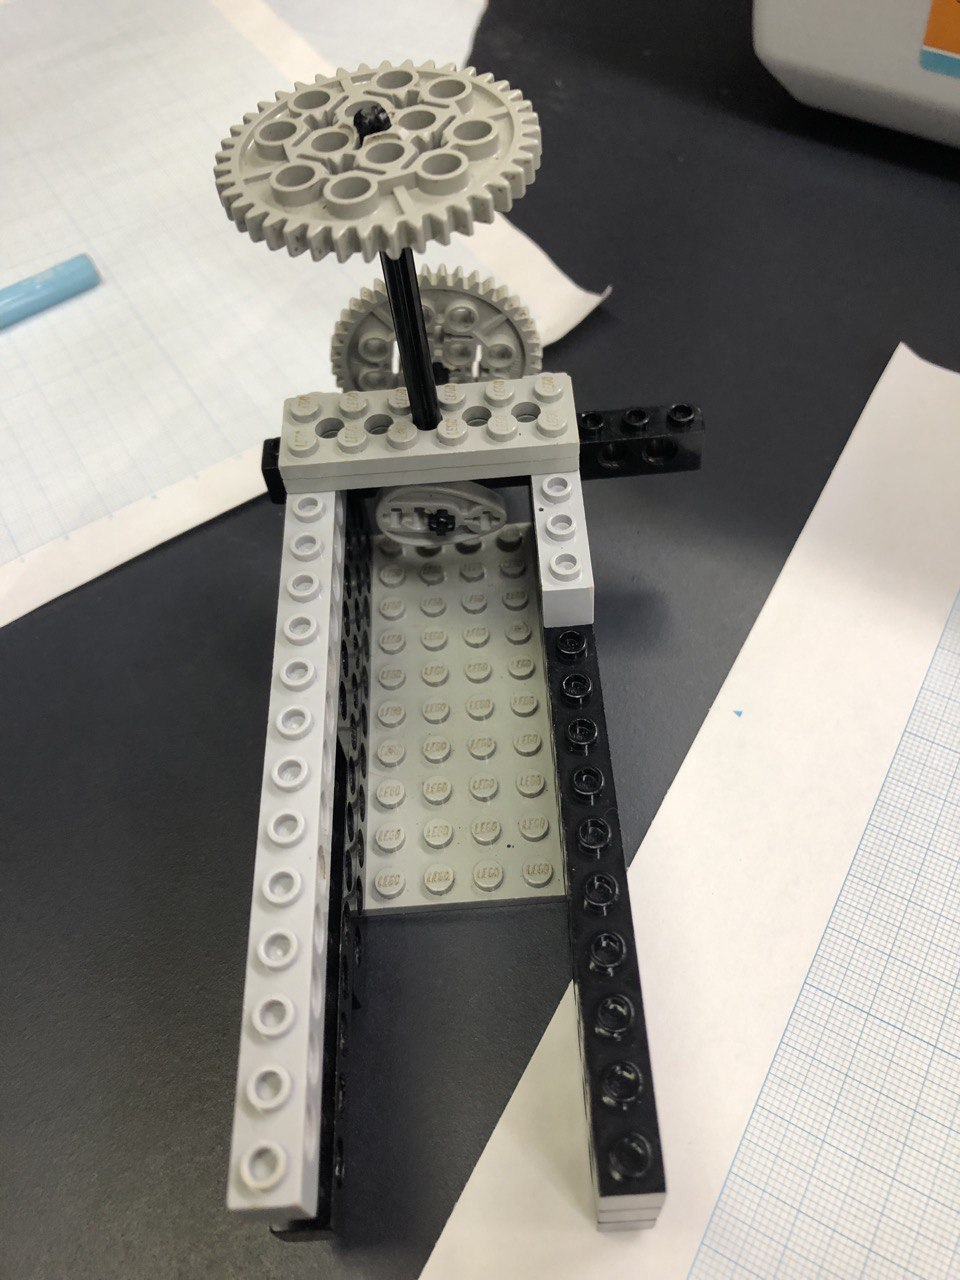
\includegraphics[width=0.5\textwidth]{figures/ass14-2}
        \caption{Figure illustrating a Cam Mechanism.}
        \label{fig:ass14-2}
    \end{figure}

    \item Slider Crank Mechanism (Figure~\ref{fig:ass14-1})\\
    A slider-crank mechanism comprises a crank, connecting rod, and slider. The crank provides rotary motion, 
    transmitting it to the connecting rod, which, in turn, imparts linear motion to the slider.
    \begin{figure}[htbp]
        \centering
        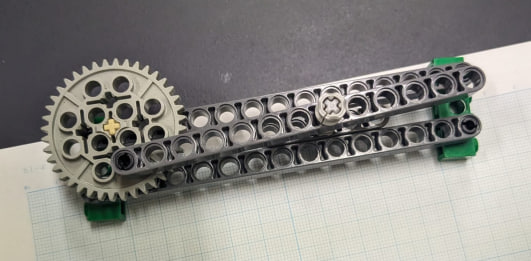
\includegraphics[width=0.5\textwidth]{figures/ass14-1}
        \caption{Figure illustrating a Slider-Crank Mechanism.}
        \label{fig:ass14-1}
    \end{figure}
\end{itemize}
\subsection{\textbf{Assignment 15}}
\begin{figure}[htbp]
            \centering
    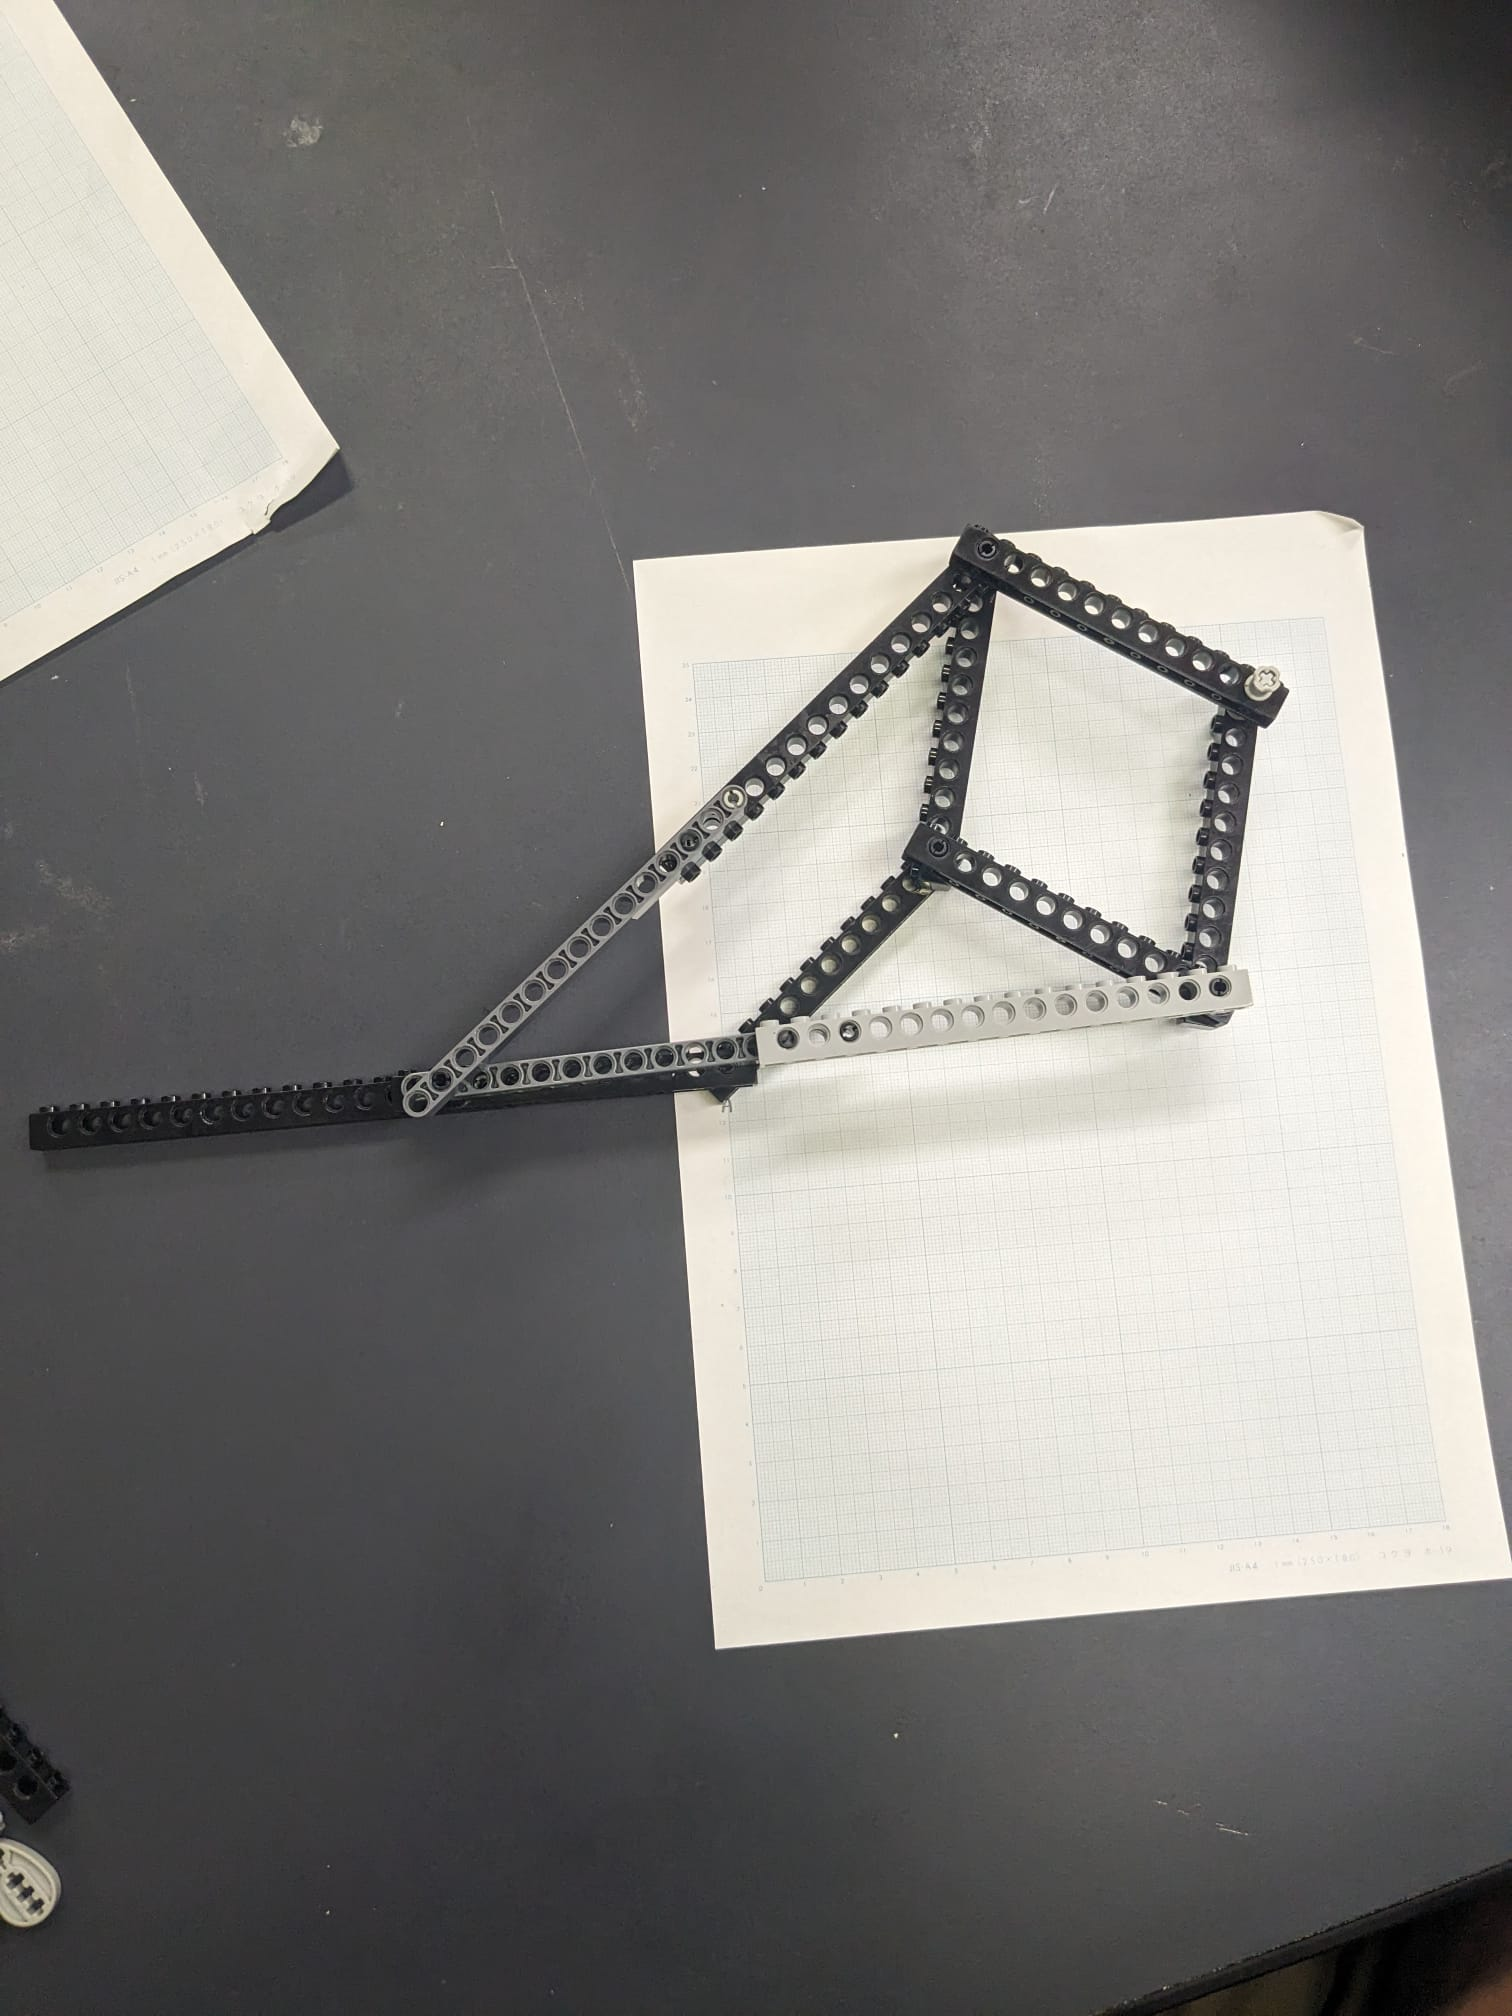
\includegraphics[width=0.7\textwidth]{figures/ass15}
    \caption{Physical structure of the Paucellier exact straight line motion Mechanism}
    \label{fig:ass15}
\end{figure}
Now, we will discuss the Paucellier exact straight line motion mechanism. The diagram for such a mechanism is illustrated in 
Figure~\ref{fig:ass15-1}. 
\begin{figure}[htbp]
        \centering
    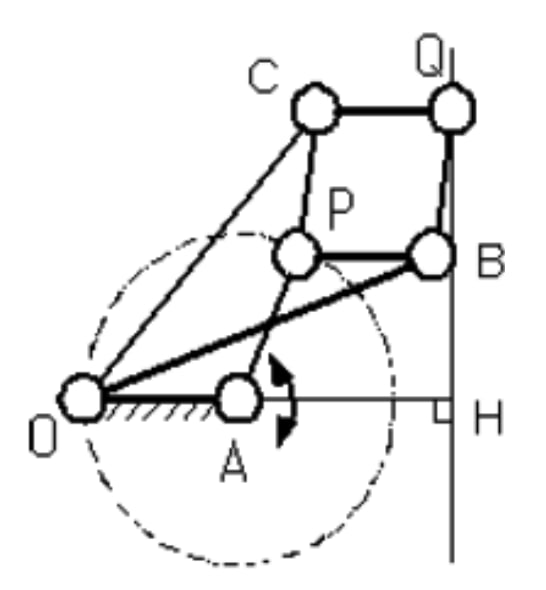
\includegraphics[width=0.7\textwidth]{figures/ass15-1}
    \caption{Figure illustrating Paucellier exact straight line motion mechanism.}
    \label{fig:ass15-1}
\end{figure}
In this assignment we prove geometrically that the point Q in Figure~\ref{fig:ass15-1} moves in a straight line. \\
See Figure~\ref{fig:ass15-1}, we can see many different triangles. 
Here, \(\Delta OBC, \Delta PBC, \Delta QBC\) are isosceles triangles. Therefore, \(OPFQ\) is a straight line. 
\begin{align}
    OP\cdot OQ &= (OF-PF)\cdot (OF+PF),\\
               &=OF^2-PF^2,\\
               &=(OC^2-CF^2)-(PC^2-CF^2),\\
               &=OC^2-PC^2=\text{ constant.}
\end{align}
Also, we see that \(\Delta OPD\) and \(\Delta OHQ\) are similar triangles. 
Thus, from property of similar triangles, we have: 
\begin{align}
    \frac{OP}{OD}&=\frac{OH}{OQ},\\
    OD\cdot OH&=OP\cdot OQ=\text{ constant.}
\end{align}
Hence proved, point Q in Figure~\ref{fig:ass15-1} will move in a straight line.  
\subsection{\textbf{Assignment 16}}
In this assignment, we make use of the Paucellier straight line mechanism and record the path of point Q on graph paper 
as in Figure~\ref{fig:ass16}. We can confirm its operation and verify that the point Q does indeed move in a straight line. 
\begin{figure}[htbp]
        \centering
    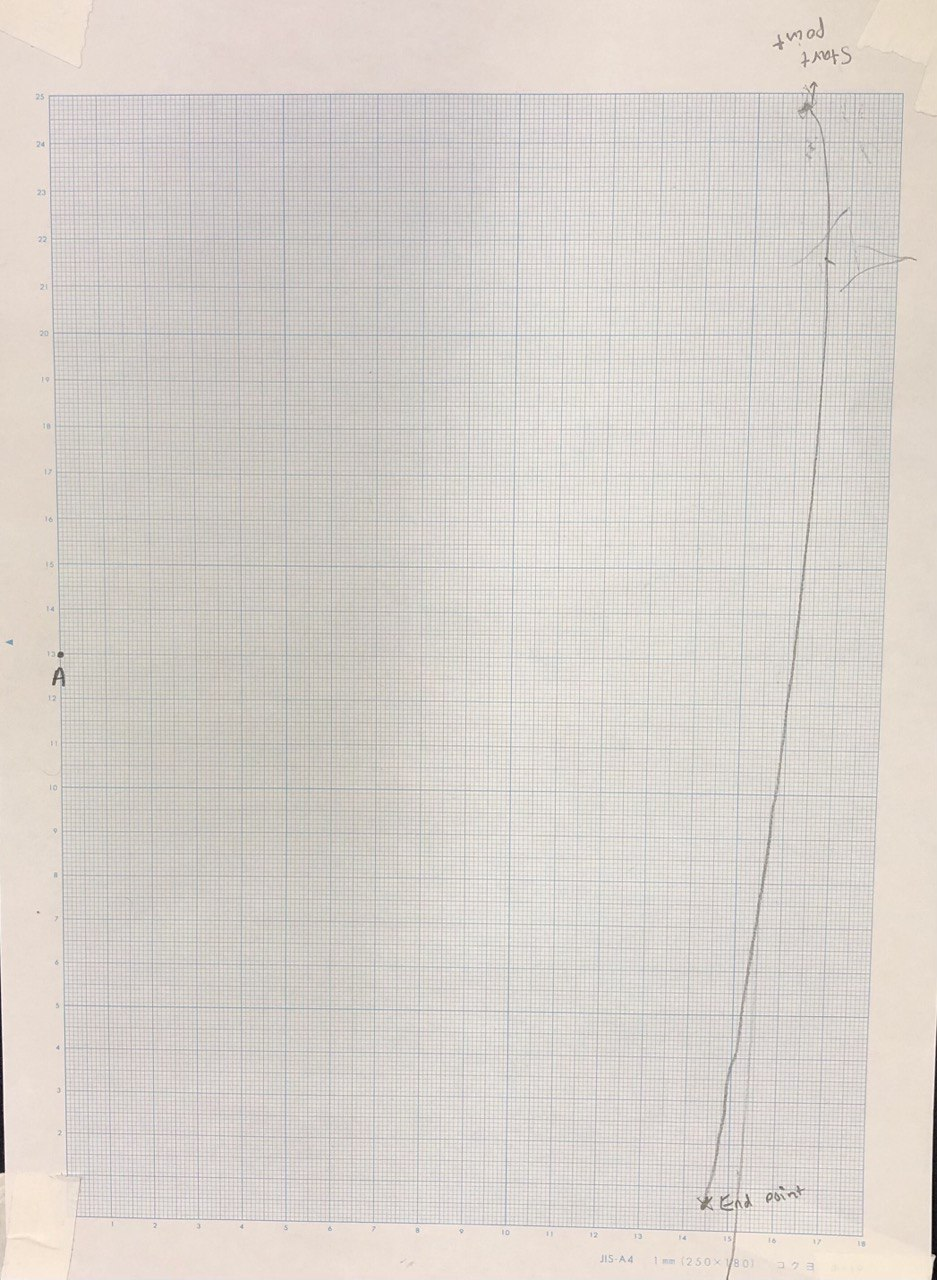
\includegraphics[width=0.7\textwidth]{figures/ass16.jpg}
    \caption{Path of point Q of the Paucellier straight line motion mechanism.}
    \label{fig:ass16}
\end{figure}
\section{Motion control using sensor}
\subsection{\textbf{Assignment 17}}
Using the aforementioned types of sensor and the motor, we build a mechanism for rotating a long beam by \(90^{\circ}\). 
We use two touch sensors, and the principle that when the motor rotates the long beam from \(0^{\circ}\) to \(90^{\circ}\), 
at the end of \(90^{\circ}\) we put a touch sensor, which gets pressed by the beam. This sensor then triggers the motor to rotate 
backwards. Now, the beam again completes moving from \(90^{\circ}\) back to \(0^{\circ}\) where it hits another touch sensor. 
This, then triggers the motor to again change directions. And just like this the beam keeps on rotating, and changing direction 
every \(90^{\circ}\). We can look at the physical mechanism in Figure~\ref{fig:ass17-1} and the program for this mechanism 
can be seen in Figure~\ref{fig:ass17-2}. 
\begin{figure}[htbp]
        \centering
    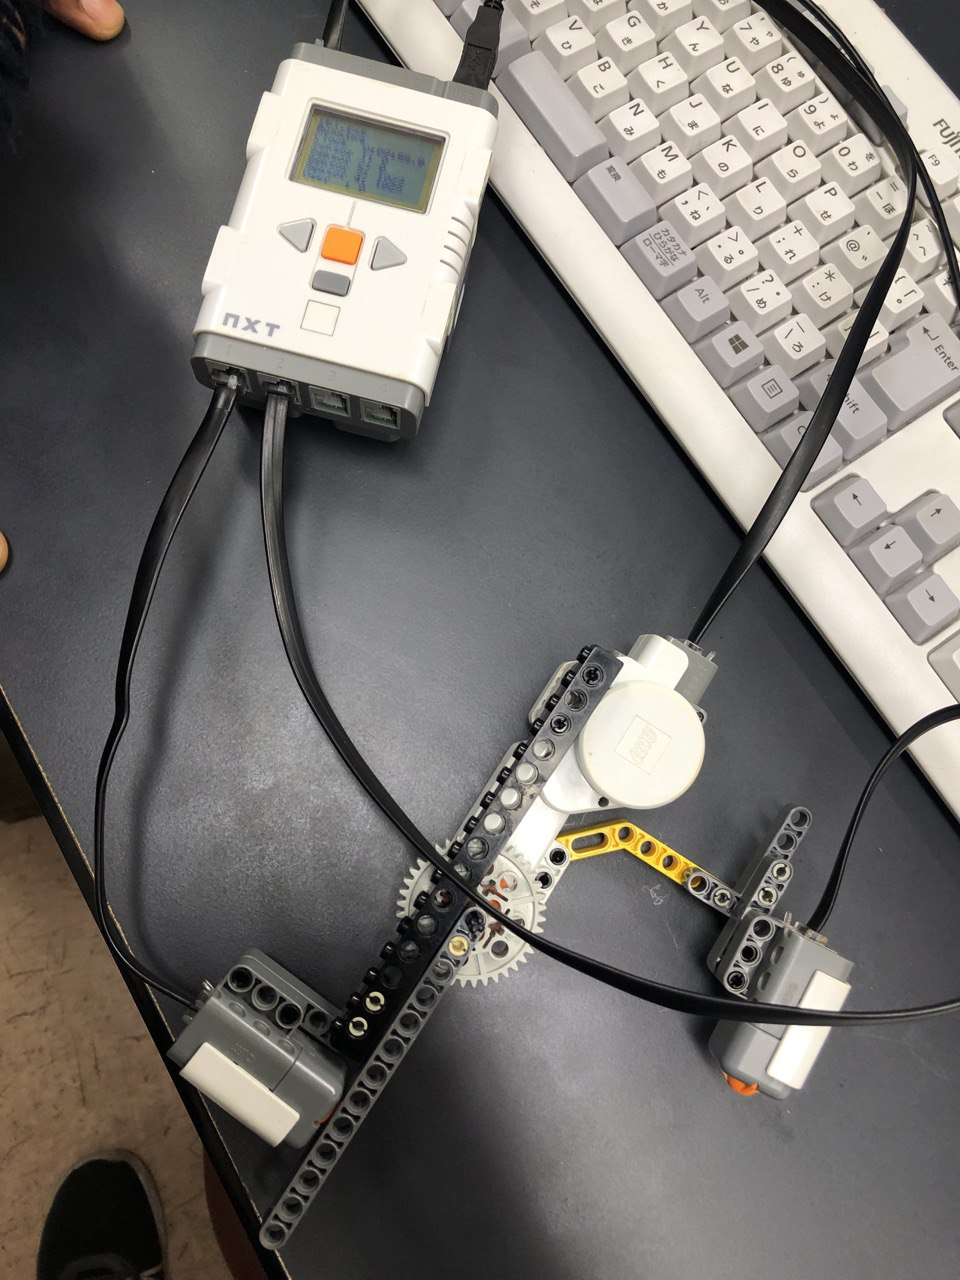
\includegraphics[width=0.7\textwidth]{figures/ass17-1}
    \caption{Physical structure of the mechanism for rotating a long beam by $90^{\circ}$.}
    \label{fig:ass17-1}
\end{figure}
\begin{figure}[htbp]
        \centering
    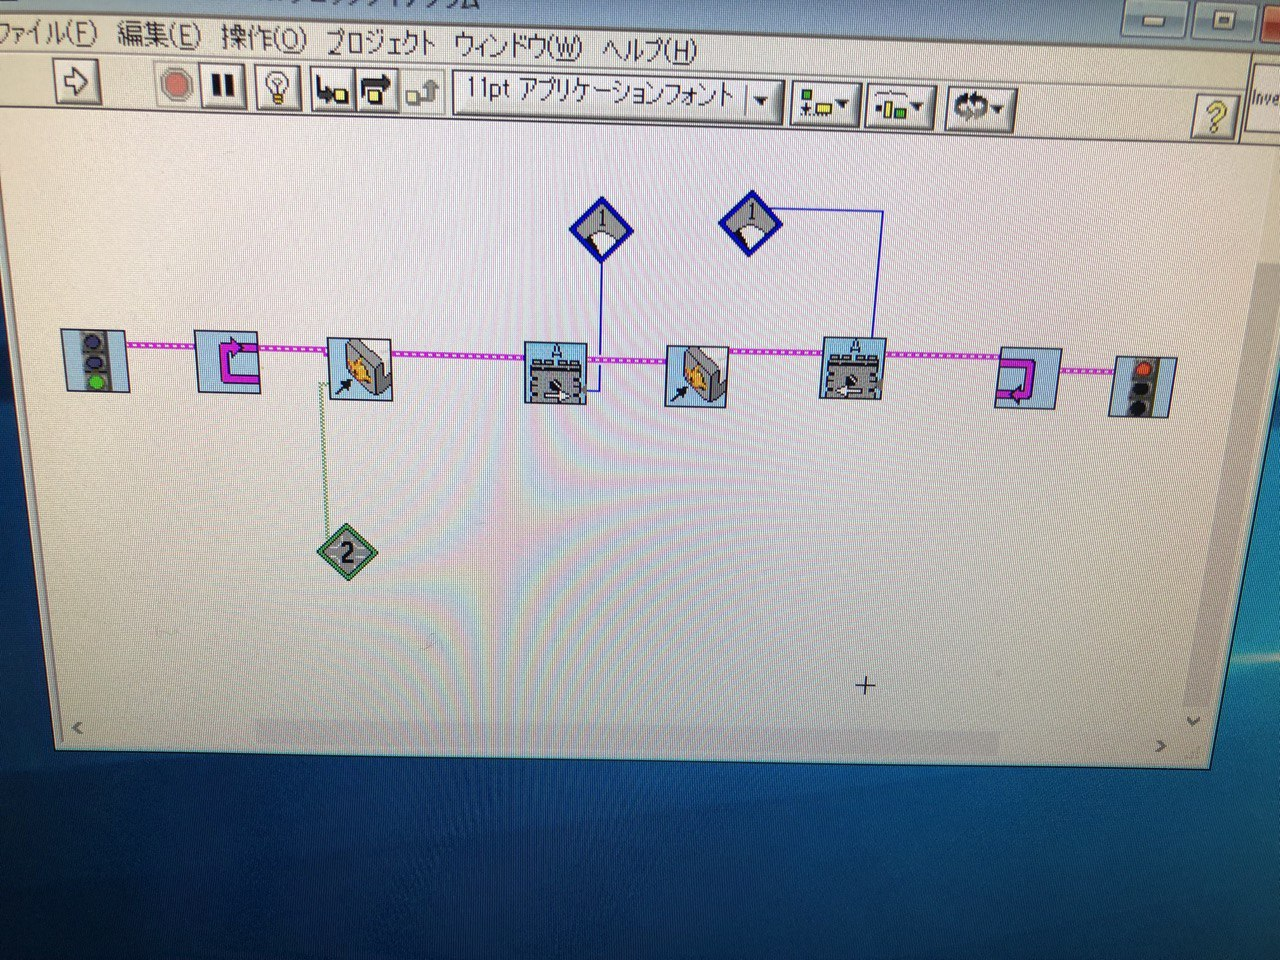
\includegraphics[width=0.7\textwidth]{figures/ass17-2}
    \caption{Program for a mechanism for rotating a long beam by $90^{\circ}$.}
    \label{fig:ass17-2}
\end{figure}

\section{Conclusion}
The series of experiments provided valuable insights into the fundamentals of Kinematics and Mechatronics. 
We covered the parallel four-link mechanism, motion conversion mechanisms, gear systems, reduction ratio, and practical 
experiments with motors and gears. We learned about how these concepts affect rotational velocity and force transmission in 
mechanical systems, providing valuable insights into engineering applications. We understood a lot of new things and it 
added to our knowledge base and provided us with experience with Robolab and making mechanisms using LEGO Mindstorms. 

\listoffigures

\end{document}
